\documentclass[12pt]{article}
\usepackage[affil-it]{authblk}
\usepackage{verbatim}
\usepackage{graphicx}
\usepackage{float}
\usepackage[utf8]{inputenc}
\usepackage[top=2.5cm, bottom=2.5cm, left=1.5cm, right=1.5cm]{geometry}
\usepackage{graphicx}
\usepackage{color}
\usepackage{float}
\usepackage[small,bf]{caption}
\setlength{\captionmargin}{3pt}
\usepackage{multicol}
\usepackage{blindtext}
\usepackage{geometry}
\usepackage{subfigure}
\usepackage{enumerate}
\usepackage{scalefnt}
\usepackage{lipsum}
\usepackage{enumitem}
\setlist{nosep} 

\title{Analysis of the STCP transport network}
\author{Diogo Bogas \\ 
        up201202482@fc.up.pt \\ 
        Departamento de Ciências de Computadores\\
        Faculdade de Ciências da Universidade do Porto\\
        }
\date{\today}


\begin{document}
\maketitle
\pagenumbering{arabic}

\begin{abstract}



\begin{center}
Abstract\\
\end{center}

This article is the final product of a study on a transport network that operates in the city of Porto, as a complex network.\\ 
I started by creating a way to extract all the information considered usefull automatically. Then upon deciding on how to store it locally, more data was derived about the network. Some of this data was derived as an input for gephi, some was generated by it. Then i present an analisys on the network, relative to degree distribution, and charateristic patters, along with the interpretation of the results obtained.


Keywords: transport network, complex networks

\end{abstract}

\begin{multicols}{2}
\section{Introduction}
% complex networks definition, example and source
In the real world, lots of information can be represented by complex networks. Some examples are chemical systems, neural networks, the Internet and the World Wide Web\cite{boccaletti2006complex}.To better understand the initial phase of this study, i introduce here two fundamental concepts.\\
%definition of xmlhttp requests and source
The first one is XMLHttpRequests. The XMLHttpRequest is an interface that allows scripts to perform HTTP client functionality, such as submitting form data or loading data from a remote Web site\cite{van2007xmlhttprequest}.
%definition of JSON and source
The next concept that the reader should be aware of is JSON. JSON stands for JavaScript Object Notation, and is a lightweight, text-based,language-independent data interchange format\cite{crockford2006application}. Knowing this, we introduce the network that this article focuses on.
% aspects to study on the network
% talvez uma referencia a distritos
% AQUI -> tenho que falar em grande porto mas n sei se hei de traduzir
%(c) Falar um bocadinho de redes de transportes 
% e do caso do Porto
In Porto, the most influential public transport company is STCP. The bus network is large enough to cover the entire city and some peripheral areas that are part of the district.\\
%(d) Falar um pouco que não existe nenhuma rede "prś-disponível" e por isso que foi necessário ir buscar
To be able to say anything about this network, first and foremost, i started searching on where to collect the data from. Ideally, some sort of database was optimal, but the most reliable place to get information ends up beeing the site, as it has lots of information usefull to this study, and it is updated regularly, as there can be alterations to the network, justifiable with construction works in some street used by it.
%(e) Falar um bocadinho do tipo de análise que fizeste
After having solid information, the analysys done consists mainly on degree distribution and charateristic patterns about the gathered information, and on facts derived from it.
%([opcional - f) explicar a organização do artigo
This article begins by exposing some relevant concepts to understand exactly how the information was colleted, and why it is reliable.\\
Then, in a separate section, it begins by explaining said gathering, continues by solving the storage problem and finally describes what type of processing was done, and to what end.\\
Then, in the Results section, all the analisys done on the network is shown, along with the interpretation of the results.

\section{Data Gathering and Processing}

\subsection{Data source}
The first decision made in this study wasn't what to study about the network, was to know were to get the data. \\
%meter referencia ao site aqui!
	The website of the company has a dropdown box that allows us to pick a random line, and shows us all the stops it goes through, and a map made with a google maps API.\\
At first, webscraping was the route followed. Web scraping \cite{vargiu2012exploiting} is  the set of techniques used to automatically get some information from a website instead of manually copying it.

 Altough this seemed to solve the problem, i found that it wasn't efficient, as i had to ,manually, iterate through the options presented and provide the HTML as input to a piece of code. Not beeing automatic , it would be painfull to update our information at any given time.
% meter referencias para os requests tambem
% aqui refiro as respostas, o que elas tem e algum thought process
The best way to do it, is to read the answers the server gives the client when an option in the dropbox is selected. Luckily, this answer is in form of JSON objects, which can be processed with some ease.\\
% referencia a resposta com todas as linhas
The first answer i took a look at, had a list of all the options on the dropdown box. This meant all the lines this company has operating were there.\\
Something important to refer, is that each line has two directions. For example: one of the lines, line 207, circulates between two stops, Campanhã and Mercado da Foz. It can start in Campanhã and go to Mercado da Foz and vice versa. While doing so, it may or may not go through the same stops, as there are one way streets in Porto that the line may use. To have accurate data, 207 by itself can't be a bus line. However, 207 in direction 0 can, as 207 in direction 1.\\
% referencia a resposta com todas as paragens da linha
The next answer had an array of all the stops that line went through. At this point, iterating through all the lines, we could know all the stops in the network.\\
% referencia a pagina de cada paragem
While looking at a line, if we click on a stop, we are redirected to a page that describes it. The same technique we used for the lines, we can use here. \\

% explicar automaçao de data gathering
The parsing of the answers the server sends the site is fully automated, using the JAVA programming language, folowing the next line of thought:

\begin{enumerate}
\item read the answer that gives all the lines
\item for each line : store it locally and collect all the stops
\item for each stop colected : get the details and store them
\end{enumerate}

About the tecniques used, it is still needed to mention the reliability of each one, and why the technique used is far superior.\\
	The method used follows a 3 steps line of thought that gives us every piece of information about the network, is automatic and takes at most ten minutes.\\
	Webscraping would follow the same algorithm, although it would envolve manual input of data, which would take much more than five minutes, and is prone to errors, as there are almost 130 different lines and close to 2500 stops.\\
	
The information the site gives about bus stops and bus lines is enough for the common user, but we need more. There are some aspects we need to derive if we want to do a complete study on the proposed network. Therefore, every piece of information was locally stored.

\subsection{Data storing}
While reading the information from the server answers, i noticed that each time i wanted to refresh my data, the running time of the script in charge of that was approximately 5 to 10 minutes. To test some methods that depended on that input, that wasn't viable. 
So, a simple answer was to create two .txt files with the information gathered.

One of the files (AllLines.txt) has all the information about each bus line.
Each bus line is represented in a single line by a code, a direction, an integer that tells us the total number of stops in that line, and finally, all the stops that compose said line.

The other file (AllStops.txt) has all the information about all the stops.
Each stop is represented in a single line by a stop code, an address, a zone, a name and a pair of floating point numbers that represent it's geographical location. 

All of this information can be refreshed, as there are methods that do so.\\

There is the need for some structures in which to represent all this data we have, so it can be easily used to answer some of the questions raised above. The first type of information stored was information about lines, and the structure to represent a line is called BusLine:
\begin{itemize}
\item Direction
\item Code
\item Description
\item Pubcode
\item LineStops
\end{itemize}
Direction is an integer that can take the values 0 or 1 and represents the direction a bus goes through a line.\\
Code is the server way to tell bus lines from each other.\\
Description is a String that tells us what appears in front of a bus that if going through a line.\\
PubCode is the people's way to tell lines from one another.\\
And LineStops is a List of Strings that represents the Stops that compose a line.\\

After knowing each line's composing stops, a list of all the stops was constructed, and the info for each stop was stored locally. The JAVA structure used is called Stop:
\begin{itemize}
	\item StopCode, the ID of a Stop.
	\item Address.
	\item Zone, the part of the city a Stop belongs to.
	\item Name, the way people know which stop is which.
	\item Longitude.
	\item Latitude.
\end{itemize}

Thinking of this network as a graph, we already have the nodes in form of stops. Now we need to derive the edges. The edges are derived from the lines, taking into account the order each line goes through the stops it serves.The Edge structure used here is as follows:

\begin{itemize}
	\item source;
	\item target;
	\item desc;
	\item weight;
\end{itemize}

Source and Target define the edge, as the network is a directed graph. Desc is a String composed by both source and target stopcodes and the weight variable represents the number of lines that use that edge. 

To make this a more complete study, the stops were grouped by 2 characteristics, the first being their address. In this case, each street was a node, and an edge represents a trip between the streets of two stops. The node is represented by the BusStreet structure:

\begin{itemize}
	\item street
	\item stops, a list of all the stops in that street
	\item longitude;
	\item latitude;
\end{itemize}

The edges in this type of grouping are represented by AdressEdge:
	
\begin{itemize}
	\item src
	\item dest
	\item weight
	\item nome
\end{itemize}
	
The graph is directed still, weight is the number of lines that use that particular interaction and nome is a way to differentiate the edges, and is derived from the source and target streets.\\

The final type of grouping was by code prefix, which is easier to explain by an example:\\
In the AllStops.txt file there are two stops which stopcodes are TSL1 and TSL2. These were grouped in a single object that is named TSL. The structure to store this type of node is called Spot:

\begin{itemize}
	\item code
	\item stops
	\item LinesServed
\end{itemize}
	
Code is the way to tell Spots apart,stops is a list of stops the Spot has in itself and LinesServed is a list with all the lines that go through that Spot.\\ 
The edges here are called SpotEdge:\\

\begin{itemize}
    \item from
    \item to
    \item weight
    \item name
\end{itemize}

"from" and "to" are the source and target Spots, weight and name, as the other types of edges are the number of lines that use the edge and a way to distinguish the edges respectively.\\
Some files, six to be more precise, were not included in this subsection, as they were generated with JAVA to be used by gephi.These files are described in the next subsection as the respective generating methods.

\subsection{Data processing and input creation}
	
	As mentioned before, Gephi was used to study the network. Gephi is a pretty powerful tool, but it requires some form of input. In this particular case .csv files. This subsection describes the methods that process the data (stored in any way described in the previous subsection) and generate the input Gephi needs.\\
	Still on the previous subsection, it was mentioned that there were 6 files left to describe. Three of these are groups of nodes, and the other three, groups of edges.\\
	
	
The first file to be described is called stops.csv , and it represents every single stop there is in this network. Five columns per stop :
	
	\begin{itemize}
		\item Id , is the code of each stop (the unique attribute).
		\item Address
		\item Zone
		\item name
		\item latitude
		\item longitude
	\end{itemize}
	
	To make this file, the method makeNodesCSV was created.
	It begins by printing "Id;Address;Zone;Name;Longitude;Latitude" in the first line of the output file. Then, for each stop it reads from the allStops.txt file, prints its attributes by the order sugested in the first line. As in the source file, each stop only takes one line.
	
	The second file to talk about is called allEdges.csv, with four columns per edge:
	
	\begin{itemize}
		\item Source stop
		\item Target stop
		\item type which is going to be directed for every edge in this study
		\item weight 
	\end{itemize}
	
	The generating method to this file is allEdgesCSV, and is similar to the nodes one.
	It also begins by printing what each column represents, (in this case "Source;Target;Type;Weight") and then for each edge it receives, prints its attributes in the order required.\\
	% paragens por rua aqui
    Because the stops were also grouped by address, we need two more files for that, the node file for that grouping is called streetNodes:\\
    \begin{itemize}
    \item Id
    \item totalStops
    \item longitude
    \item latitude
    \end{itemize}
    
    This first file is generated by the makeStreetNodeCSV method, which in the first line of the file writes "Id;TotalStops;Longitude;Latitude", and in each subsequent line writes each streetNode's values. \\
   And the edges file is called streetEdges:\\
   \begin{itemize}
   \item weight
   \item source 
   \item target 
   \item type
   \end{itemize}
    The second file for this type of grouping  is generated by makeStreetEdgesCSV, and this file holds, for each edge, the weight, source, target and type.The weight in this particular case represents how many bus lines use that particular edge.\\
    
	%paragens por code aqui
	The last type of grouping is by code prefix. This allows us to group spots that are near each other (and potentially have a similar name ) in a single structure we call Spot:
\begin{itemize}
	\item code
	\item stops
	\item LinesServed
\end{itemize}
	
Code is the way to tell Spots apart,stops is a list of stops the Spot has in itself and LinesServed is a list with all the lines that go through that Spot.\\
The code variable derivation is easy to exemplify: in our list of Stops there are two whose codes are TSL1 and TSL2. These were grouped in a Spot which code is TSL.

The edges in this type of grouping are represented by the SpotEdge structure:
\begin{itemize}
\item from
\item to
\item weight
\item name
\end{itemize}

From and to are the source and target Spots, weight and name, as the other types of edges are the number of lines that use the edge and a way to distinguish the edges respectively.
	
\section{Results}
	To better understand the results obtained, i'm introducing the final two concepts.
	The first one is betweeness centrality. Betweeness measures how many times a cenrtain node acts as a bridge on the shortest path between two other nodes. On another words, it tells us how "central" each node is.\\
	The last concept is excentricity. This represents the longest shortest path that can be measured starting at a certain node.	\\
	This first image is the very first piece of information that our tool gave us, a visual representation of all 2416 stops in the network(not using any type of grouping), colored by zone. All of these stops interact between them a total of 2823 times to create 142 lines. Using the GeoLayout i got:\\

\begin{figure}[H]
	\centering
	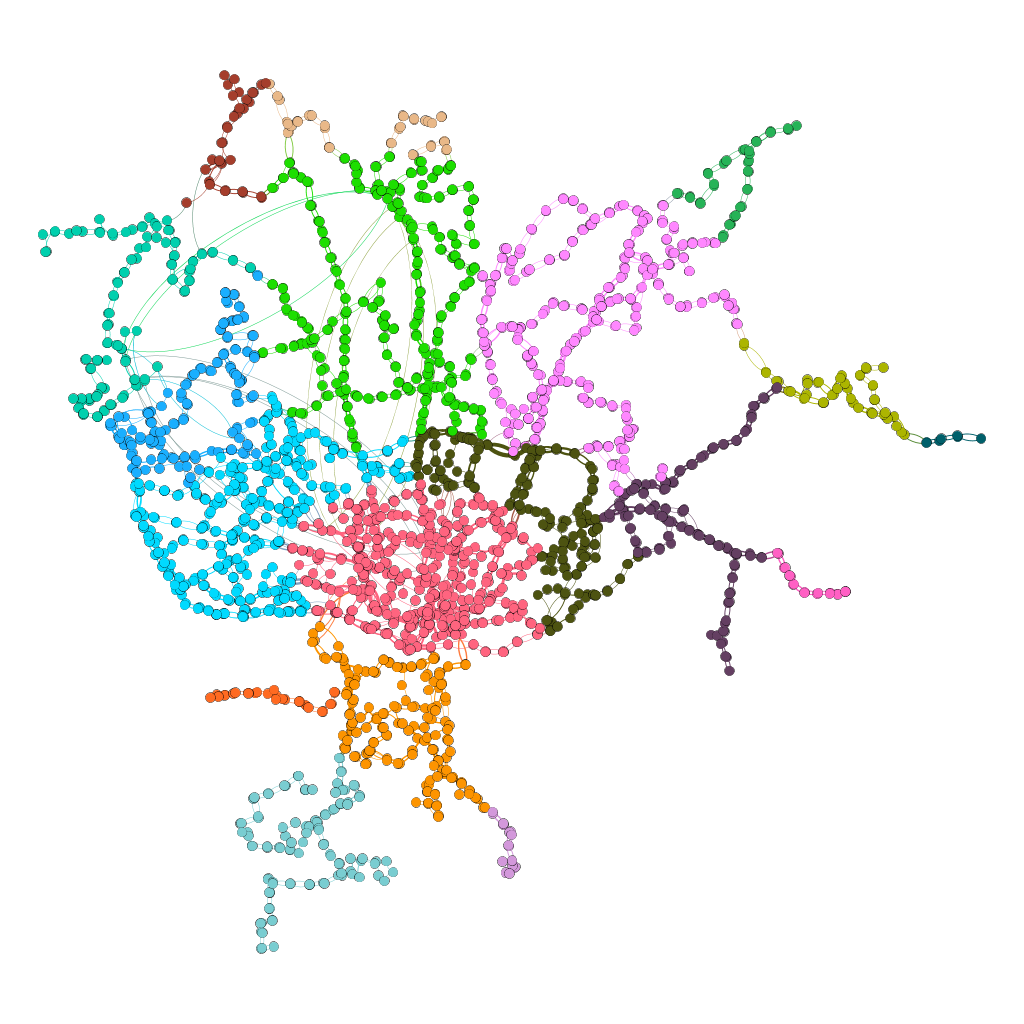
\includegraphics[scale=0.2]{simple_network}
	\caption{The network, without grouping, with stops colored by zones and shown according to geographical coordinates}
\end{figure}
The following image is the palette used to color the network shown above, and it ends up giving us how large is each zone relatively to it.\\
\begin{figure}[H]
	\centering
	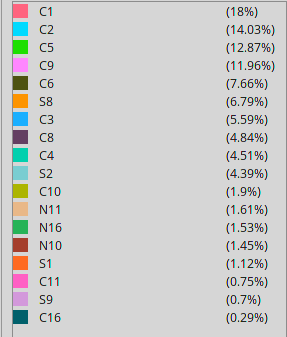
\includegraphics[scale=0.5]{legenda_simples}
	\caption{A table with all the zones, sorted according to size,displaying each zone's color}
\end{figure}

Here is displayed the top 10 in terms of excentricity:\\
\begin{tabular}[h]{|l|l|}
\hline
Stop & Excentricity\\
\hline
Rio Tinto (Estação) & 136.0	\\
Cabine & 135.0\\
Perlinhas & 135.0\\
José Poças & 134.0\\	
José Portugal & 134.0\\
Lourinha & 134.0\\
Cedofeita & 133.0\\
Monte & 133.0\\
Piscinas & 133.0\\	
Bicheiros & 132.0\\
\hline
\end{tabular}\\
% sim eu ainda vou explicitar como calculei as duas pontas do caminho
% aqui exponho a excentricidade para o grafo ""simples
The eccentricity table was extracted from Gephi's data laboratory, and we now know the stop that has the largest excentricity, or in another words, one end of the network diameter. But, what about the other end of that shortest path? It's relatively easy to discover as the diameter of a network can be calculated using a Breath First Search. The other end's stop is named Cabine. In this case the two stops on top of the table are the farthest away from each other.Although, this is not allways true to all networks.\\
% aqui falo da betweeness para este grafo
In terms of Betweeness centrality, the most "central" nodes are the following:
\begin{center}
\begin{tabular}[h]{|l|l|l|}
\hline
Zone & name & Betweeness\\
\hline
C1   & Trindade	& 1145449.881\\
C1	 & Graciosa	& 771297.511\\
C1	 & Boavista Cemitério & 754319.608\\
C1	 & Moreira Sá & 736031.847\\
C6 	 & Asprela & 678387.028\\
C1	 & Av.Aliados & 644478.771\\
C1	 & Trindade & 612273.626\\
C6	 & IPO(Circunval.)	& 611095.614\\
C6	 & Areosa	& 601167.850\\
C1	 & Boavista-Casa da Música	& 583327.933\\
\hline
\end{tabular}
\end{center}

There is a pattern that relates betweeness and the zone each stop belongs to. Looking to the table above,  most stops there belong to zones C1 and C6. This happens because C1 is the center of the city, and C6 contains lots of stops near Universities.\\
One question the reader can raise is: "Which Stop has the most lines going through it and how many times?". For this, it's better to group the stops by code, and answer a different question : "Which Spot has the most lines going through it?", as a Spot is much more influential than a simple Stop. The answer to this, is in the table below,extracted from spotNodes.csv where the 5 most populated Spots are represented:
% degree distribution to spots
\begin{center}
\begin{tabular}[h]{ |c|c|c| }
\hline
    Id  & totalStops & linesServed\\
    \hline
    Trindade & 6  & 21 \\
    Casa da Música & 5 & 20 \\
    Bom Sucesso  & 8 & 18 \\
    Aliados & 6 & 17 \\
    Carmo & 4 & 17 \\
\hline
\end{tabular}
\end{center}
% betweeness to spots
Betweeness:
\begin{center}
\begin{tabular}[h]{|l|r|}
\hline
Zone & Betweeness\\
\hline
Asprela & 186589.726494106\\
Areosa & 169476.566820944\\
Sá e Melo  & 160771.644333675\\
Trindade & 142065.711680429\\
Sra.Penha & 140319.297660562\\
Exponor & 138773.349901777\\
Av.Vasco da Gama & 138042.401294208\\
Pego Negro & 137306.819005155\\
Sta. Luzia & 134573.103619802\\
S.Roque & 134205.67288033\\
\hline
\end{tabular}
\end{center}
% excentricity to spots
Excentricity:\\
\begin{center}
\begin{tabular}[h]{|c|c|}
\hline
Spot & Eccentricity\\
\hline
MAKRO &	33\\
Gaia Shopping & 33\\
Rua do Senhor & 34\\
Quatro Caminhos	& 34\\
Telheira & 34\\
Rua Sr.Matosinhos & 34\\
AKI & 34\\
Sra.Penha & 35\\
Alex Herculano & 35\\
Batalha & 35\\
\hline
\end{tabular}
\end{center}


In terms of streets, we want to know what is the street that holds the most stops. Checking the streetNodes.csv file and sorting by descending order the totalStops column, its verified that Estrada da circunvalação holds 86 stops. After some fact checking, it was verified that this street is 17 km long[2], which justifies a 64 stops difference to the 2nd street in this ranking. Follows the top 5:
%degree distribution to streets
\begin{center}
\begin{tabular}[h]{|l|c|}
\hline
Street & Total Stops\\
\hline
Estr.Circunvalação & 86\\
R.D.Afonso Henriques & 32\\
Av.Boavista	& 30\\
R.S.Vicente& 23\\
R.Costa Cabral & 22\\
\hline
\end{tabular}
\end{center} 

% Betweeness
Analising betweeness in this case, only serves to validate what was exposed about streets before about the degreee distribution:\\
\begin{center}
\begin{tabular}[h]{|l|r|}
\hline
Street & Betweeness\\
\hline
Estr.Circunvalação	& 144958.4586 \\
R.D.Afonso Henriques &	84015.0718\\
Av.República &	77292.4868\\
R.5 Outubro	& 61082.3386\\
R.Rodrigues Freitas &	47389.2129\\
R.Júlio Dinis	& 46894.5706\\
Av.Boavista &	45395.5349\\
R.Pádua Correia &	44121.7983\\
R.Guerra Junqueiro &	40522.3095\\
Av.Fernão Magalhães &	33811.9214\\

\hline
\end{tabular}
\end{center}

% excentricity to Streets
In terms of excentricity i got this table:
\begin{center}
\begin{tabular}[h]{|l|l|}
\hline
Street	& Eccentricity\\
\hline
R.Prof.Manuel Cardoso Ribeiro & 29\\
R.Pena & 28\\
Rot. Natália Correia & 27\\
R.Rodelo & 27\\
R.Gestalinho & 26\\
R.Julião Sarmento &	26\\
R.Alto Chaquedas & 26\\
R.Ponte Do Carro & 26\\
R.P. Abílio Sampaio & 25\\
R.Boa Hora & 25\\
\hline
\end{tabular}
\end{center}

\section{Conclusion}
	The results that we obtained colide with the reality.It was expected that the centre of Porto was the most busy zone of the entire network, and proof of that, is that C1 is the biggest zone,and most of it's Stops have the biggest Betweeness in the entire graph. The prior knowledge i had about the service this company provides, and the city itself, helped me as a "sanity check" as the data was processed. This study also allowed me to get a deeper understanding of Graph theory , and it's applications in real life situations.

\begin{comment}
\section{References}
[1] Albert-László Barabasi, Network Science\\[0pt]
[2] https://pt.wikipedia.org/wiki/EN12
\end{comment}

\bibliographystyle{acm}	
\bibliography{report}
\end{multicols}	
\end{document}